\part{System Design and Methodology}

% \textbf{NOTE:}
% Included here is the system architecture and explanation of each process. Discuss
% how each problem was developed and \textbf{where the algorithm will be used} in
% solving the problem.

\begin{figure}[hbt!]
	\center
	\noindent\adjustbox{width=\textwidth}{\includesvg{images/salitrato_colored_flowchart}}
	\caption{SaLitrato process flowchart}
	\label{fig:salitrato_flowchart}
\end{figure}

\section*{Design Goal Overview}

\hspace\parindent
The figure (Fig \ref{fig:salitrato_flowchart}) above illustrates how the system software that implements an in-image text search method will search for and extract text within an image or multiple image files using Boyer-Moore algorithm. A text pattern within an image file will be detected and located using the Boyer-Moore algorithm. The system will additionally incorporate the use of optical character recognition (OCR) API with the version of Tesseract 4 to identify and extract texts from images.

\hfill

The user will create and select a folder to which the pre-processed file would be stored, the aforementioned file would then be checked if it is one of the supported formats. It will then be subjected to the Python Tesseract package where it will undergo a connected component analysis that gathers and stores the outlines. The outlines will then be further analyzed in a fixed pitch or if they are proportional texts. They will then be separated into words according to character spacing by using character cells.

\hfill

Lastly it will undertake a two-pass procedure using an adaptive classifier to enhance the accuracy of the recognition process. Only then will it be put through the Boyer-Moore Algorithm where the user-inputted characters will be compared to the text from the post-processed file. To be able to assist the users easily identify the result, the software also has a feature that highlights the location of the text pattern inside an image file or displays a prompt if the pattern is not recognized.

\section*{System Architecture}

\hspace\parindent
This software is built using a modular, object-oriented approach with focus on readability,
maintainability, and extensibility. It follows the traditional \texttt{layered architecture}, with
several layers managing the user interface, application logic, and system interactions.

\begin{figure}[hbt!]
    \center
    \noindent\adjustbox{width=\textwidth}{\includesvg{images/archpat}}
    \caption{System architecture of SaLitrato}
    \label{fig:plannedUI}
\end{figure}

\section*{Data Storage Design}

\hspace\parindent
On initial start of the application, the user is met with the selection of add, open, and remove
folder. Every folder created is stored in the current working directory (\texttt{\$CWD}) of where 
the application was executed. This specifically appears on the \texttt{data/} folder which
can be located at \texttt{\$CWD/data/$<$folder\_name$>$}.
Inside \texttt{\$CWD/data/$<$folder\_name$>$}, is where the extracted text from an image will be
stored. The CSV file is also generated here replicating the name of its current folder 
(\texttt{$<$folder\_name$>$.csv}). This acts as a database of current selected image files to 
be run on by the Boyer-Moore Algorithm.

\begin{center}
\begin{tabular}{| c | c | c |}
    \hline
    \texttt{file\_key} & \texttt{file\_path} & \texttt{file\_name}\\
    \hline
    1 & \texttt{\textasciitilde/Projects/filename1.png} & filename1.png\\
    \hline
    2 & \texttt{\textasciitilde/Photos/filename2.jpeg} & filename2.jpeg\\
    \hline
    3 & \texttt{\textasciitilde/Downloads/images/filename3.jpg} & filename3.jpg\\
    \hline
    4 & \texttt{\textasciitilde/Projects/filename5.webp} & filename5.webp\\
    \hline
\end{tabular}
\end{center}

\section*{Data Structure Preparation for Indexing}

\begin{figure}[hbt!]
    \center
    \noindent\adjustbox{width=.95\textwidth}{\includesvg{images/data_format}}
    \caption{Structure of data for processing}
    \label{fig:data_structure1}
\end{figure}

\hspace\parindent
In figure \ref{fig:data_structure1}, it shows how the data will be structured. This prepares the
text of each file to undergo what we call as indexing. Indexing refers to identification of the
location of a resource based on file names or key data fields in a record. Traversing through a
record like this (Fig \ref{fig:indexing}) would make tracking the index of where the pattern appeared become easier.

\begin{figure}[hbt!]
   \center
   \noindent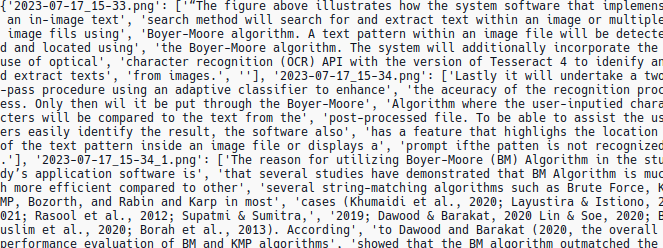
\includegraphics[width=\textwidth]{row_data.png}
   \caption{Sample data}
   \label{fig:indexing}
\end{figure}

\section*{Algorithm}

\hspace\parindent
Having multiple lists of text to traverse through requires a fast and efficient algorithm for
pattern matching. There were multiple string matching algorithms existing like Naive Algorithm, Z
Algorithm, Knuth Morris Pratt, and Boyer Moore algorithm.  Observing that
as the number of image files being included for search increases, the number of text to be passed by
the algorithm also increased drastically. Among said stiring matching algorithms,
\textbf{Boyer Moore string matching algorithm} works best in this kind of scenario. Though at worst
case it runs on $O(nm)$ where n is the length of text and m is length of pattern, it is outweighed
by its best case of $O(n/m)$ assuming there are limited number of matches occured which happens to
be the case on having multiple texts to traverse.

\hfill

The \textbf{Boyer Moore Algorithm} in this program uses bad character heuristics to determine where
the mismatch appeared. Multiple references exist for getting the code for this algorithm, but it
comes with several drawbacks. We take the example of what was written in GeeksForGeeks [21]. 

\hfill

\begin{lstlisting}
NO_OF_CHARS = 256
 
def badCharHeuristic(string, size):
    badChar = [-1]*NO_OF_CHARS
    for i in range(size):
        badChar[ord(string[i])] = i;
    # returns bad_char_array

def search(txt, pat):
    badChar = badCharHeuristic(pat, m)
    # return indexes of where the patterns appeared
\end{lstlisting}

\hfill

When this type of code is executed, multiple instances of \texttt{badChar} will be recreated for
every row there is to search for a match. This ramps up the complexity by increasing orders of
magnitude. The \texttt{badCharHeuristic()} function itself can get $O(size)$ as its complexity.
Without refactoring the code, it could reach a complexity of $O(size*rows)$ given the data is now
being traversed. It can be
prevented by decoupling \texttt{badCharHeuristic()} inside the \texttt{search()}. Making the search
contain the \texttt{badChar} only as an argument.

\hfill

Another problem for the code shown above is the \texttt{NO\_OF\_CHARS = 256}. Giving a limit to the
values that can be inserted into the bad character array, would most likely generate an \texttt{Out
of Bounds Exception} or
\texttt{IndexError}. The said error is raised when an index that is out of range or invalid for
a given data structure is being accessed. Making this array a hash table is one of the solution. Instead of being
allocated manually and limiting the extension of bad character array, it becomes dynamically allocated on its own.

\hfill

\begin{lstlisting}
def badCharHeuristic(pat):
    table = {}
    for i in range(len(pat)):
        table[pat[i]] = i
    return table
\end{lstlisting}

\noindent
\texttt{\{'a': 0, 'n': 1, 'd': 2\}} - sample pattern input: "and"

\hfill

\section*{Retrieval of Matched Patterns}
Getting the result of matches occured requires the algorithm to traverse on multiple list of
rows on each file while retrieving the current index of where each pattern started.
